\documentclass{beamer}

%
% Common preamble for all three parts.
%

\usepackage[spanish]{babel}
\usepackage{amsmath}
\usepackage{color}
\ProvidesPackage{minted}
\usepackage{minted}
%\setminted{encoding=utf8}
\usepackage{hyperref}
\usepackage{multicol}
\usepackage{tabularx}
\usepackage{tikz}

\usepackage[utf8x]{inputenc}
%\usepackage{ucs}
%\usepackage[T1]{fontenc}
%\newcommand{\minted@encoding}{\minted@get@opt{encoding}{UTF8}}

% o Warsaw, Bergen, Madrid, ...
%\usetheme{Berkeley}
\usetheme{Warsaw}

% o albatross, beaver, crane, ...
% \usecolortheme{whale}
\definecolor{IUAblue}{RGB}{53,62,91}
\definecolor{IUAamarillo}{RGB}{254,187,80}


\setbeamercolor*{palette primary}{use=structure,fg=white,bg=IUAblue}
\setbeamercolor*{palette quaternary}{fg=white,bg=IUAamarillo}%black!30!IUAamarillo}

%\setbeamercolor{structure}{bg=IUAamarillo, fg=IUAamarillo!90!IUAblue}

% no nav buttons
%\usenavigationsymbolstemplate{}

\newcommand{\bftt}[1]{\textbf{\texttt{#1}}}
\newcommand{\comment}[1]{{\color[HTML]{008080}\textit{\textbf{\texttt{#1}}}}}
\newcommand{\cmd}[1]{{\color[HTML]{008000}\bftt{#1}}}
\newcommand{\bs}{\char`\\}

%\logo{
\includegraphics[width=.125\textwidth]{images/logo_f_azul}}



\title{Servicios Web}
\author{Franco Bocalon \and Luis Guanuco \and Santiago Nolasco}
\institute[ESE -- IUA]{Especialización en Sistemabas Embebidos \\
  Instituto Universitario Aeronáutico}
\date{29 de Abril del 2016}
\titlegraphic{%

\includegraphics[width=.2\textwidth]{images/logo_f_blanco}
}

\subtitle{Sistemas Distribuidos}

\begin{document}

%%%%%%%%%%%%%%%%%%%%%%%%%%%%%%%%%%%%%%%%%%%%%

\begin{frame}
  \titlepage
\end{frame}

%%%%%%%%%%%%%%%%%%%%%%%%%%%%%%%%%%%%%%%%%%%%%
\section{Introducción}
%%%%%%%%%%%%%%%%%%%%%%%%%%%%%%%%%%%%%%%%%%%%%

\begin{frame}
  \frametitle{Contenidos}
  \tableofcontents[currentsection,hideallsubsections]
\end{frame}

\begin{frame}{\insertsection{}}
  \frametitle{Arquitectura Orientada a Servicios (SOA)}
  Plantea una organización de recurso de forma que una colección
  desordenada de sistemas distribuidos y aplicaciones complejas se
  transformen en una red de recursos integrados, simplificados y
  sumamente flexible.
  \vfill
  \centering
  \footnotesize
  \begin{tabular}{|l|l|}
    \hline
    \textbf{Arquitectura tradicional} & \textbf{Arquitectura orientada
      a servicios}\\
    \hline\hline
    Forzada a la funcionalidad & Orientado al proceso \\\hline
    Diseñado para durar & Diseñado para el cambio\\\hline
    Desarrollo con largos ciclos de tiempo & Desarrollo
    iterativo\\\hline
    Fuerte acoplamiento & Bajo acoplamiento \\\hline
    Aplicación especifica & Heterogéneo\\\hline
    Orientado a datos & Orientado al servicio empresarial\\
    \hline
  \end{tabular}
\end{frame}

\section{Servicios basados en SOA}

\begin{frame}
  \frametitle{Contenidos}
  \tableofcontents[currentsection,hideallsubsections]
\end{frame}

\begin{frame}{\insertsection{}}
  \frametitle{Principal uso}
  \centering
  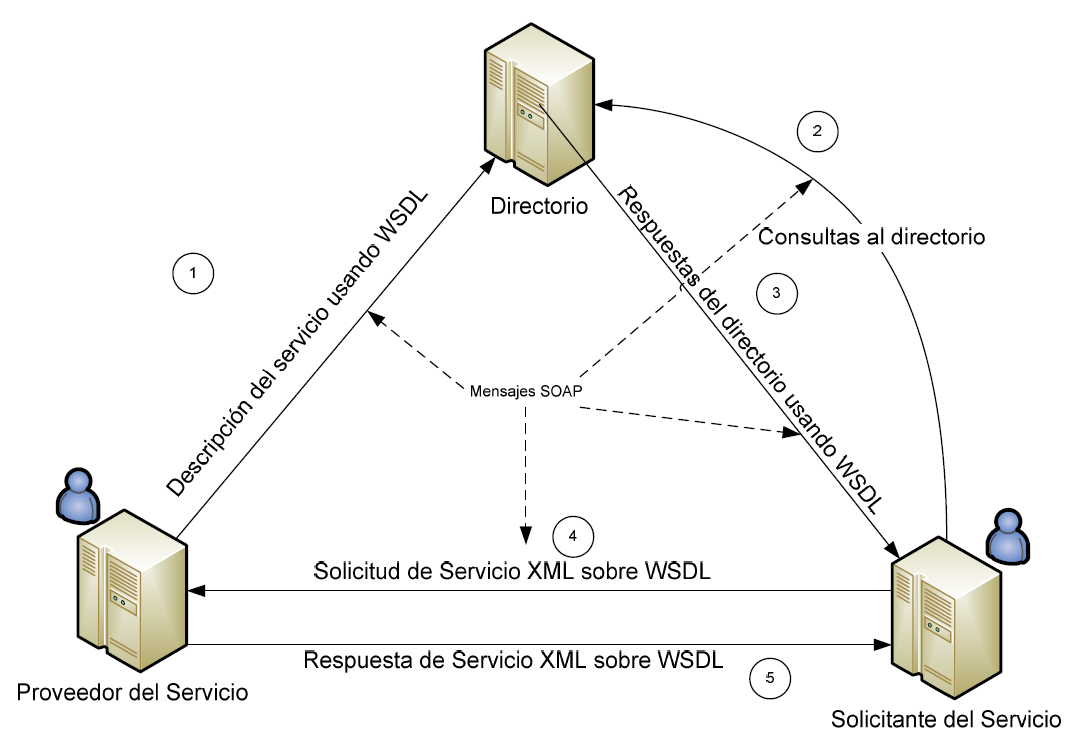
\includegraphics[width=.9\textwidth]{images/img-from-paper/soa.jpg}
\end{frame}

\begin{frame}{\insertsection{}}
  \frametitle{Estándares}
  \begin{description}
  \item[XML:] Permite definir la gramática de lenguajes
    específicos para estructurar documentos grandes.
  \item[WSDL:] Basado en XML, describe la forma de
    comunicación (protocolos, formatos, etc.) con los servicios
    ofrecidos.
  \item[SOAP:] Utilizado para el intercambio de datos. La base de este
    protocolo son: \emph{Extensibilidad}, \emph{Neutralidad} y
    \emph{Independencia}.
  \end{description}
\end{frame}

\begin{frame}{\insertsection{}}
  \frametitle{SOAP}
  El enfoque de SOAP es encapsular la lógica como solicitud de la base
  de datos para el servicio. 

  \vfill

  \centering
  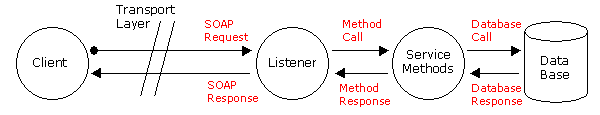
\includegraphics[width=\textwidth]{images/img-from-paper/soap-comp.jpg}
\end{frame}

\section{REST}

\begin{frame}
  \frametitle{Contenidos}
  \tableofcontents[currentsection,hideallsubsections]
\end{frame}

\begin{frame}{\insertsection{}}
  \frametitle{Orígenes}
  En el 2000 Roy
    Fielding\footnote{\burl{https://es.wikipedia.org/wiki/Roy_Fielding}}
    presenta el estilo de arquitectura REST. Lo define como un estilo
    híbrido derivado de otras arquitecturas con la \emph{aplicación de
    restricciones a cumplir}.
  \\~\\
  Las restricciones planteadas por Fielding buscan mejorar las
  características deseadas en las arquitecturas Web modernas. 
\end{frame}

\begin{frame}{\insertsection{}}
  \frametitle{Restricciones de REST}
  \begin{description}
    \only<1>{\item[Client-Server:] La independencia del cliente hacia el
      servidor (y recíprocamente) permite la implementación de \emph{múltiples
        plataformas} desde el lado del cliente, y la \emph{escalabilidad}
      por el lado del servidor.}
    \only<2>{\item[Stateless:] El servidor no debe almacenar ninguna
      información sobre el contexto del cliente en sus llamadas.}
    \only<3>{\item[Cache:] Mejorar la eficiencia de la red. Lo
      importante en esta restricción es proporcionar información
      suficiente para saber \emph{qué} almacenar para ser
      reutilizado.}
    \only<4>{\item[Uniforme Interface:] Una de las características
      centrales de REST, que lo distingue de otras arquitecturas, es
      el énfasis en una \emph{interfaz uniforme} entre componentes.}
  \end{description}
  \vfill{}
  \centering 
  \includegraphics<1>[scale=.5]{images/client_server_style}
  \includegraphics<2>[scale=.5]{images/stateless_cs}
  \includegraphics<3>[scale=.5]{images/ccss_style}
  \includegraphics<4>[scale=.5]{images/uniform_ccss}
\end{frame}


\begin{frame}[fragile]{\insertsection{}}
  \frametitle{Un simple ejemplo -- SOAP}
  Se pide obtener datos de un usuario a partir de su
  identificador. Usando la arquitectura \emph{SOAP}, la petición mediante
  \texttt{HTTP POST} tendría la forma:

  \begin{lstlisting}
    <?xml version="1.0"?>
    <soap:Envelope
    xmlns:soap="http://www.w3.org/2001/12/soap-envelope"
    soap:encodingStyle="http://www.w3.org/2001/12/soap-encoding">
    <soap:body pb="http://www.acme.com/phonebook">
    <pb:GetUserDetails>
    <pb:UserID>12345</pb:UserID>
    </pb:GetUserDetails>
    </soap:Body>
    </soap:Envelope>
  \end{lstlisting}

  La respuesta la almacena el cliente, podría ser un archivo XML, y
  la respuesta al pedido se encuentra embebido en el mensaje.
\end{frame}

\begin{frame}[fragile]{\insertsection{}}
  \frametitle{Un simple ejemplo -- REST}
  Sí el servidor implementa RESTfull, la consulta anterior se hace con
  el URL de abajo. Aquí con el comando \texttt{HTTP GET} obtenemos la
  respuesta en bruto.

  \begin{lstlisting}
    http://www.acme.com/phonebook/UserDetails/12345
  \end{lstlisting}

  Aquí el método REST es \texttt{UserDetails} en vez de
  \texttt{GetUserDetails}. Esto se debe a la convención del diseño de
  REST donde se usa \emph{sustantivos} en vez de \emph{verbos} para
  referirse a un \emph{recurso}.
\end{frame}

\section{Comparación de Servicios Web}

\begin{frame}[fragile]{\insertsection{}}
  \frametitle{Principales diferencias}
  \centering
  \footnotesize
  \bgroup
  \def\arraystretch{1.8}%  1 is the default, change whatever you need
  \begin{tabular}{m{5cm}m{5cm}}
    \textbf{SOAP} & \textbf{REST}\\
    Orientado a la manipulación  de objetos remotos. & Orientado a la
    aplicación de operaciones sobre los recursos. \\\pause
    Demanda mayor flujo de datos en comparación con REST. & No requiere
    un mapeo total de los objetos. \\ \pause
    Madurez y robustez en su estructura. & Flexible y fácil de
    implementar.\\ \pause
    Implementación de WS* para empresas & Implementado actualmente en
    todos los WS públicos.\\
  \end{tabular}
  \egroup
\end{frame}

\section{Conclusiones}

\begin{frame}[fragile]{\insertsection{}}
  \frametitle{Conclusiones desde nuestra perspectiva}
  
  \begin{itemize}
    \setlength\itemsep{2em}
  \item<1-> La \emph{flexibilidad} de REST atrae a los
    desarrolladores.
  \item<2-> La propuesta de Fielding se alinea con la
    \emph{escalabilidad} de los sistemas actuales.
  \item<3-> El \emph{estado del arte} de los WS* apunta a las
    arquitecturas ROA (REST Oriented Architecture). La industria web
    mudo hace tiempo todos sus sistemas a \emph{RESTful}.
  \end{itemize}
\end{frame}

\appendix{}

\section{Veamos un ejemplo}

\begin{frame}[fragile]{\insertsection{}}
  Se implementa un simple WS* con \emph{RESTful}. Vamos a
  realizarle pedidos...
  \vfill
  
  \begin{lstlisting}
    http://localhost:8080/SISTEMASDISTRIBUIDOS/RESTDEMO/...
  \end{lstlisting}

\end{frame}

\end{document}
